
\begin{document}

\chapter{Matiti Structure} 
\label{sec:MatitiStructure} 
In the \emph{ParticleFracturing} directory you can find a directory named as \emph{Matiti}. \emph{matiti} itself consists of other folders like: src, opt, runs and triangle as it can be seen in figure~\ref{fig:MatitiDirectoryGraph}.
\begin{figure}
  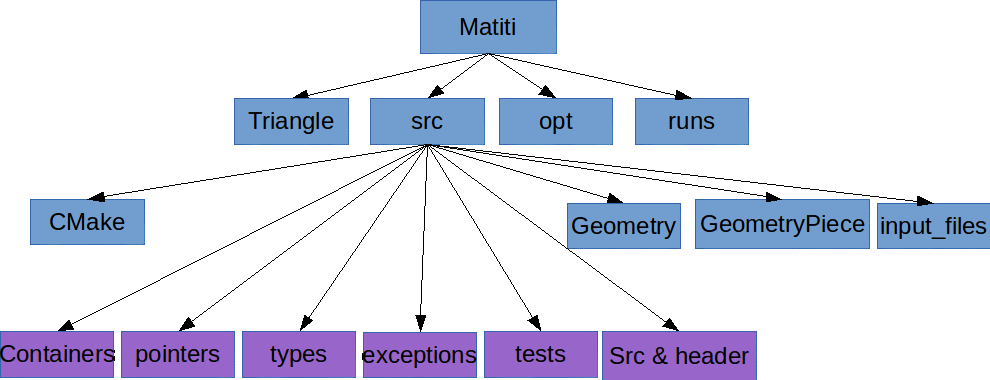
\includegraphics{MatitiDirectoryGraph.png}
  \caption{Directory Graph for Matiti}
  \label{fig:MatitiDirectoryGraph}
\end{figure}
\begin{itemize}
\item From the \emph{Triangle} directory you need a library with which you can discretize your surface into triangle shaped parts.    
\item \emph{opt} is a directory that you make in order to make the needed files such as the executable files from your source directory so you can run the program. 
\item \emph{runs} is where you run your program and save the out-put data (as vtk file format) to be visualised using a proper package like visIt. 
\item \emph{src} is the source folder where all the input files and programs are gathered in it. This directory again includes other folders and files which are categorized in figure~\ref{fig:MatitiDirectoryGraph}. \\
First group which are shown by the blue boxes are:
 \begin{itemize}
 \item \emph{CMake} finds the runtimes for cmake so you can make all the needed files out of the src directory into the opt directory.
 \item \emph{Geometry} is where simple geometries such as point, vector, box and polygon are made, figure~\ref{fig:Geometry}:
\begin{figure}
  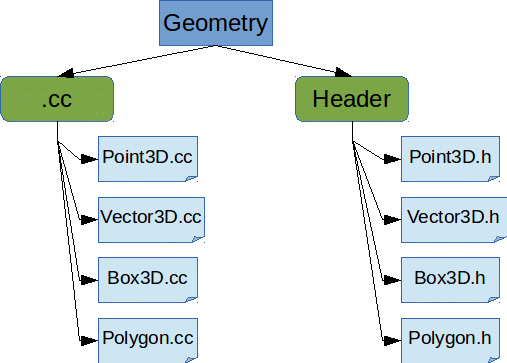
\includegraphics{Geometry.png}
  \caption{Graph for Geometry directory}
  \label{fig:Geometry}
\end{figure}
 \item \emph{GeometryPiece} is a directory in which geometry pieces can be created using two input nodes (as lower and upper) and the elementary geometries introduces in the \emph{Geometry} directory. This directory consists of files as shown in figure~\ref{fig:GeometryPiece}
\begin{figure}
  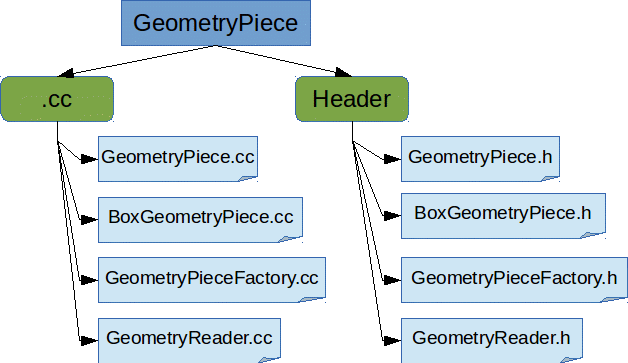
\includegraphics{GeometryPiece.png}
  \caption{Graph for GeometryPiece directory}
  \label{fig:GeometryPiece}
\end{figure}
 \item \emph{input-files} is a directory in which all your input files have been gathered. These are the files that you need to copy them into the \emph{runs} directory, whenever you want to run them, and from there run it using the executable file in the \emph{opt} directory (--> \emph{test\_peri}.) Organization and the skeleton of these input files are described in the next chapter (--> \textbf{Chapter}~\ref{chap:Organization})
 \end{itemize}
Instead of these directories, there are so many files in the src. We have made some groups shown by the violet color. These files are devided and arranged in each group based on their properties and applications:
\begin{itemize}
 \item \emph{containers} as shown in figure~\ref{fig:containers}
\begin{figure}
  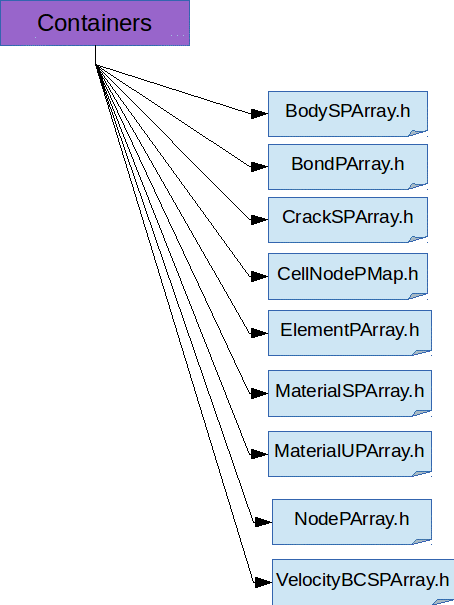
\includegraphics{containers.png}
  \caption{Graph for Containers Group}
  \label{fig:containers}
\end{figure}
 \item \emph{Pointers} as shown in figure~\ref{fig:Pointers}
\begin{figure}
  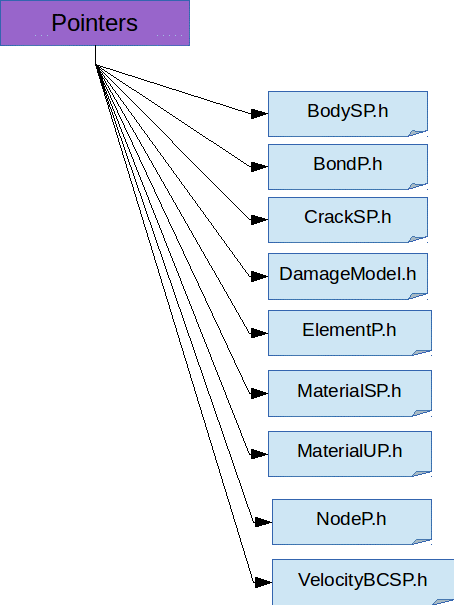
\includegraphics{Pointers.png}
  \caption{Graph for Pointers Group}
  \label{fig:Pointers}
\end{figure}
 \item \emph{Types} as shown in figure~\ref{fig:Types}
\begin{figure}
  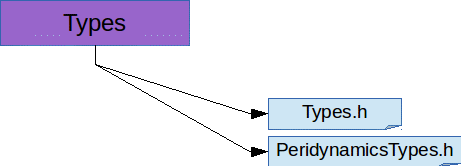
\includegraphics{Types.png}
  \caption{Graph for Types Group}
  \label{fig:Types}
\end{figure}
 \item \emph{Exceptions} as shown in figure~\ref{fig:Exceptions}
\begin{figure}
  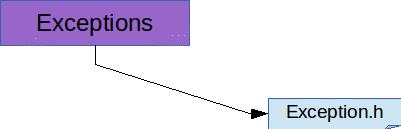
\includegraphics{Exceptions.png}
  \caption{Graph for Exceptions Group}
  \label{fig:Exceptions}
\end{figure}
 \item \emph{Tests} as shown in figure~\ref{fig:Tests}
\begin{figure}
  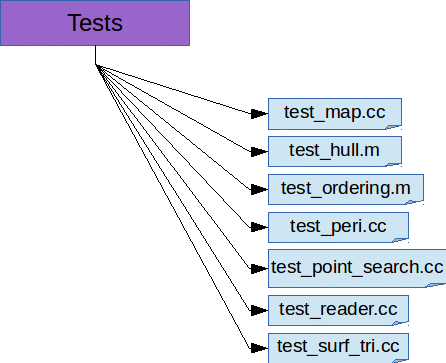
\includegraphics{Tests.png}
  \caption{Graph for Tests Group}
  \label{fig:Tests}
\end{figure}
 \item \emph{Src \& header} as shown in figure~\ref{fig:SrcAndHeader}
\begin{figure}
  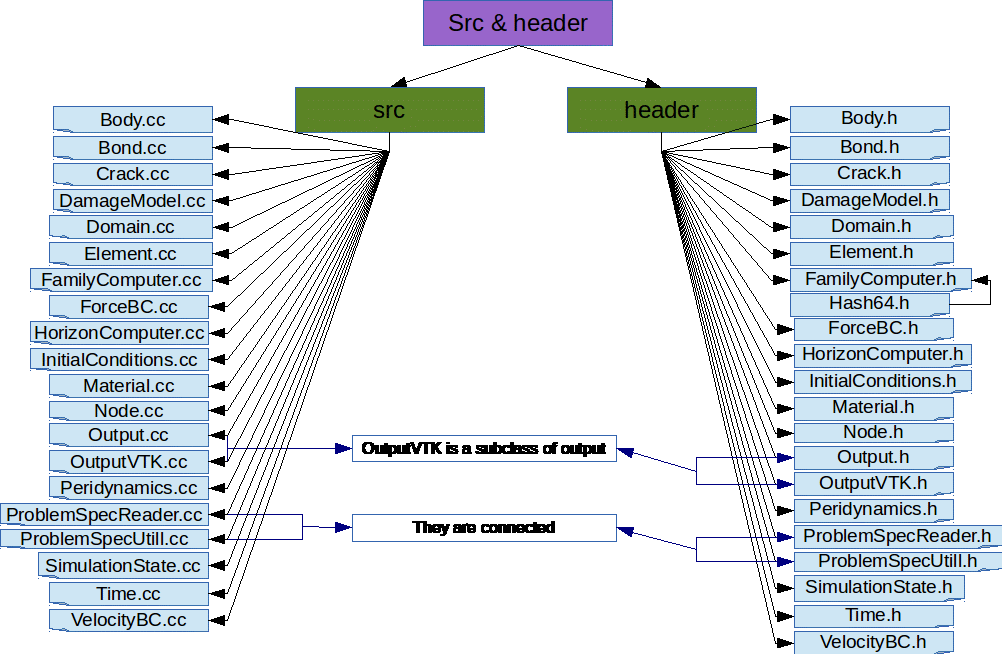
\includegraphics{SrcAndHeader.png}
  \caption{Graph for Src \& header Group}
  \label{fig:SrcAndHeader}
\end{figure}
 \end{itemize}
\end{itemize}







\chapter{Organization}
\label{chap:Organization}

The Matiti Peridynamics programs work as described below:
\begin{itemize}
\item First it gets an input using \emph{ProblemSpecReader} and \emph{ProblemSpecUtil}
\item All the calculations on the data would be done in a mainbody of the program (saved in the input files directory.) This part is called the \textbf{Domain}.
\item and the out put data would be saved as VTK files using \emph{Output} and \emph{OutputVTK} programs. 
\end{itemize}

All the above items are gathered in figure~\ref{fig:Perischem}
\begin{figure}
  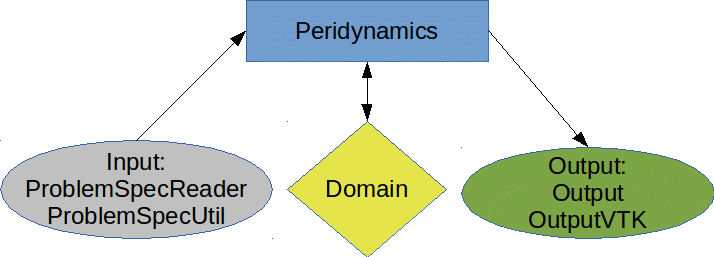
\includegraphics{Perischem.png}
  \caption{Graph for the Peridynamics schematic job}
  \label{fig:Perischem}
\end{figure}

Domain is where you can make your bodies or objects. Before the domain part, in the main body, we set the \emph{time} and \emph{Simulation State} and in the domain part, having the domain points we set the \emph{VelocityBC}. Now in the domain we can make our object(s) or the Body(s) but before that we need to make the \emph{Nodes}. \\
Actually, the \emph{GeometryPiece} makes \emph{Elements} with which we can have our \emph{Nodes}. Moreover \emph{Material} should be made using the \emph{Damagemodel} and be passed to the \emph{Nodes} through the \emph{Bond}. For making the nodes we also need \emph{FamilyComputer} and \emph{HorizonComputer} to find the neighbours of each node. (See figure~\ref{fig:Nodes})
\begin{figure}
  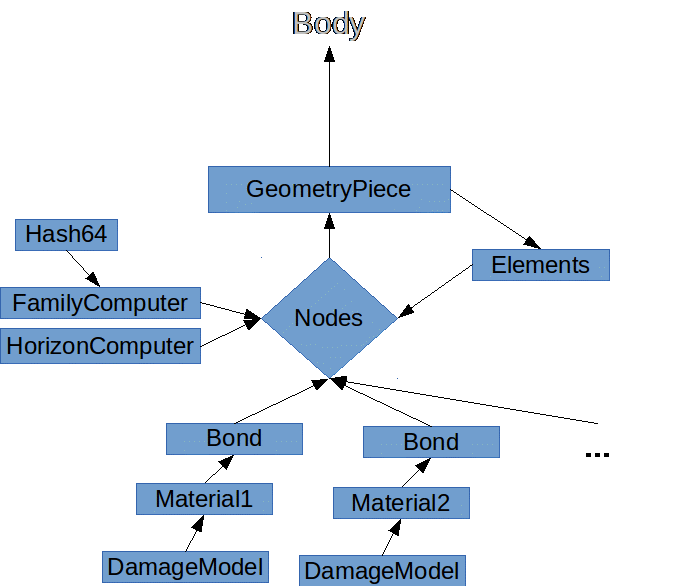
\includegraphics{Nodes.png}
  \caption{Graph for the Nodes}
  \label{fig:Nodes}
\end{figure}

Now that we have the nodes we just need to give the \emph{Initial Conditions} and \emph{Force Boundary Conditions} so we can have our body(s). The \emph{Initial Condition} is made of \emph{Cracks}, \emph{initial Velocity} and the \emph{Body Forces} like the gravity.
All the information regarding the domain structure and organization is gathered in figure~\ref{fig:Domain})
\begin{figure}
  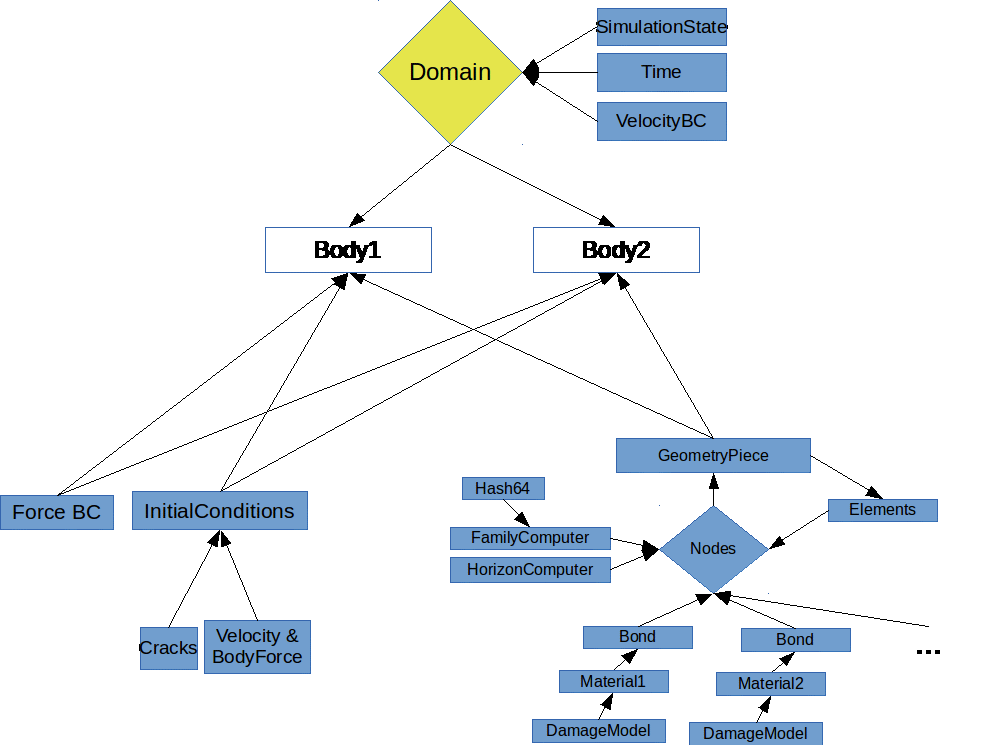
\includegraphics{Domain.png}
  \caption{Graph for the Domain}
  \label{fig:Domain}
\end{figure}



\end{document}
